\documentclass[
    type = bachelor,
    degree = academic,
    twoside,
    fontset = win,
    decl-page
]
{njuthesis}

% njuthesis 参数设置文件 v1.4.0 2024-03-19

\njusetup[info]{
    title = {面向TLA\textsuperscript{+}规约的\\归纳不变式自动生成技术},
    title* = {Automatic Inductive Invariants Learning for TLA\textsuperscript{+} Specifications},
    author = {张继华},
    author* = {Jihua Zhang},
    keywords = {TLA\textsuperscript{+}, 分布式系统, 形式化验证, 强化学习, 归纳不变式},
    keywords* = {TLA\textsuperscript{+}, Distributed System, Formal Verification, Reinforcement Learning, Inductive Invariant},
    grade = {2020},
    student-id = {201250040},
    department = {软件学院},
    major = {软件工程},
    major* = {Software Engineering},
    supervisor = {魏恒峰,助理研究员},
    supervisor*= {Hengfeng Wei, Research Assistant},
    submit-date = {2024-05-20},
    % 提交日期
    supervisor-contact = {
        南京大学~
        江苏省南京市鼓楼区汉口路22号
    }
    % 导师联系方式
}

% bib 类用于参考文献设置
\njusetup[bib]{
    % style = numeric|author-year,
    % 参考文献样式
    % 默认为顺序编码制(numeric)
    % 可选著者-出版年制(author-year)
    %
    resource = {zhangjihua-thesis.bib},
    % 参考文献数据源
    % 需要带扩展名的完整文件名
    % 可使用逗号分隔多个文件
    % 此条等效于 \addbibresource 命令
    %
    % option = {
        % doi    = false,
        % isbn   = false,
        % url    = false,
        % eprint = false,
        % 关闭部分无用文献信息
        %
        % refsection = chapter,
        % 将参考文献表置于每章后
        %
        % gbnamefmt = lowercase
        % 使用仅首字母大写的姓名
    %   }
    % 额外的 biblatex 宏包选项
}

% image 类用于载入外置的图片
\njusetup[image]{
    % path = {{./figure/}{./image/}},
    % 图片搜索路径
    %
    nju-emblem = {nju-emblem},
    nju-name = {nju-name},
    % nju-emblem = {nju-emblem-purple},
    % nju-name = {nju-name-purple},
    % 替换为紫色版本
    % 这个选项只能填写一次
    % 切换时要注释掉上方的黑色版本
}

% abstract 类用于设置摘要样式
\njusetup[abstract]{
    toc-entry = true,
    % 摘要是否显示在目录条目中
    %
    % underline = false,
    % 研究生英文摘要页条目内容是否添加下划线
    %
    % title-style = strict|centered|natural
    % 研究生摘要标题样式,详见手册
}

% 目录自身是否显示在目录条目中
\njusetup{
    tableofcontents/toc-entry = false,
    % 关闭本项相当于同时关闭三个选项
    %
    % listoffigures/toc-entry   = false,
    % listoftables/toc-entry    = false
}

% 为目录中的章标题添加引导线
\njusetup[tableofcontents/dotline]{chapter}

% math 类用于设置数学符号样式,功能详见手册
\njusetup[math]{
    % style              = TeX|ISO|GB,
    % 整体风格,缺省值为国标(GB)
    % 相当于自动设置以下若干项
    %
    % integral           = upright|slanted,
    % integral-limits    = true|false,
    % less-than-or-equal = slanted|horizontal,
    % math-ellipsis      = centered|lower,
    % partial            = upright|italic,
    % real-part          = roman|fraktur,
    % vector             = boldfont|arrow,
    % uppercase-greek    = upright|italic
}

% theorem 类用于设置定理类环境样式,功能详见手册
\njusetup[theorem]{
    % define,
    % 默认创建内置的七种定理环境
    %
    % style         = remark,
    % header-font   = \sffamily \bfseries,
    % body-font     = \normalfont,
    % qed-symbol    = \ensuremath { \male },
    % counter       = section,
    % share-counter = true,
    % type          = {...}
    % 以上设置项在重新调用 theorem/define 后生效
}

% footnote 类用于设置脚注样式,功能详见手册
\njusetup[footnote]{
  % style = pifont|circled,
  % 使用圈码编号
  %
  % hang = false,
  % 不使用悬挂缩进
}

% 页眉页脚内容设置
\njusetup{
  % header/content = {
  %     {OR}{\thepage},{OL}{\rightmark},
  %     {EL}{\thepage},{ER}{\leftmark}
  %   },
  % 页眉设置,详见手册
  % 奇数页页眉:左侧章名,右侧页码
  % 偶数页页眉:左侧页码,右侧节名
  %
  % footer/content = {}
}

% 页眉页脚的字体样式
% \njusetformat{header}{\small\kaishu}
% \njusetformat{footer}{}

% 一些灵活调整
\njusetname{type}{本科毕业设计}                 % 我做的是毕业设计
% \njusetname{notation}{术语表}                   % 更改符号表名称
% \njusetlength{crulewd}{240pt}                   % 加长封面页下划线
% \njusetformat{tabular}{\zihao{-4}\bfseries}     % 修改表格环境的字号
% \EditInstance{nju}{u/cover/emblem-img}{align=l} % 左对齐的本科生封面校徽

\usepackage{listings} % 展示代码
\usepackage{algorithm,algorithmic} % 展示算法伪代码
\usepackage{subcaption} % 嵌套小幅图像,比 subfig 和 subfigure 更新更好
\usepackage{siunitx} % 标准单位符号

\newcommand{\TLA}{TLA\textsuperscript{+}\ }

\begin{document}
% 封面
\maketitle

\begin{abstract}
    分布式协议以及分布式系统,在当今的计算机世界不可或缺。自动化地对分布式协议验证其正确性是一个重要且困难的挑战。
    为了验证分布式协议的正确性,我们可以尝试证明分布式协议的每一个状态都满足一个预先给定的不变式,即安全属性(safety property)。
    对于复杂系统,我们无法像验证简单系统,通过遍历所有状态的方式来验证安全属性。
    过去的研究中往往采用寻找一个蕴含着安全属性的不变式的方式来验证协议的正确性,这个不变式经过所有可能的状态转移后仍然能保持其自身的正确性。
    这个不变式被称为归纳不变式。
    自动化地生成分布式协议的归纳不变式是验证自动化分布式协议正确性的关键步骤。

    以往的研究主要基于的IVy进行实现,\TLA 语言领域的相关研究较少。本文将提供一种基于\TLA 的归纳不变式生成工具,实现对以\TLA 语言描述的分布式协议规约的归纳不变式的自动化生成。
    与此同时,通过引入了强化学习的方法,加速归纳不变式的推导。
    引入外部工具 \href{https://apalache.informal.systems/}{apalache} 作为验证引擎,实现了对归纳不变式的验证。
    在进入强化学习模块之前,我们基于 tla2tools 对 \TLA 源文件进行静态分析,提取出语义信息,以便强化学习框架理解 \TLA 文件的语义。
    通过实验,本文提出的方法的有效性和可行性可以得到验证。
\end{abstract}
  
\begin{abstract*}
    Distributed Protocols and distributed systems are indispensable in today's computer world. Automatically verifying the correctness of distributed protocols is an important and challenging task.
    To verify the correctness of distributed protocols, we can try to prove that every state of the distributed protocol satisfies a pre-defined invariant, a safety property.
    For complex systems, we cannot verify safety properties by traversing all states as we do for simple systems.
    Researchers often use the method of finding an invariant that implies the safety property, which remains correct after all possible state transitions. This invariant is called an inductive invariant.
    Automatically generating inductive invariants for distributed protocols is a key step in verifying the correctness of automated distributed protocols.

    Previous research is mainly based on IVy for implementation, few on \TLA. 
    This paper will provide an inductive invariant generation tool based on \TLA, which realizes the automatic generation of inductive invariants for distributed protocol specifications described in \TLA language.
    Meanwhile, it accrelerates the derivation of inductive invariants by introducing reinforcement learning methods.
    The external tool \href{https://apalache.informal.systems/}{apalache} is introduced as a verification engine to verify the inductive invariants.
    Before entering the reinforcement learning module, we perform static analysis on the \TLA source files using tla2tools to extract semantic information for the reinforcement learning framework to understand the semantics of the \TLA files.
    Through experiments, the effectiveness and feasibility of the method proposed in this paper have been verified.
\end{abstract*}

% 目录
\tableofcontents

% 正文
\mainmatter
\chapter{绪论}

\section{研究背景和意义}
分布式协议,如 Paxos和 Raft等,是现代分布式系统的基石。
验证分布式协议的正确性,对保障大规模的数据库系统,云计算系统以及其他分布式系统运行的可靠性和稳定性至关重要。
然而,目前分布式协议愈发复杂,验证分布式协议的正确性并不是一件容易的事情。
在分布式协议验证中,安全属性(safety property)具有至关重要的地位。
如果在运行过程中,系统的每个状态都不违背安全属性,那么我们可以认为这个系统是安全的。
因此,验证分布式协议的正确性,可以转化为验证系统的每个状态都满足安全属性的问题。
对于复杂系统,我们无法简单地采用遍历的方式来验证安全属性是否在每个状态下都成立。
目前的研究方式,大多是寻找一个归纳的不变式,这个不变式经过所有可能的状态转移后仍然能保持其自身的正确性。
并且,这个不变式蕴含着安全属性,即这个不变式成立,则安全属性成立。
这个不变式被称为归纳不变式\cite{inductive}。
寻找到归纳不变式就等同于验证了分布式协议的正确性。\cite{towards}
自动化地生成分布式协议的归纳不变式是验证自动化分布式协议正确性的关键步骤。

\TLA \cite{TLA+}是一个对程序和系统,尤其对并发和分布式的程序和系统进行规约建模的高级语言。
在并发和分布式系统设计和开发过程中,非常容易发生基础性的设计问题,这些问题往往难以被发现。
而\TLA 以及其工具,利用集合论和时态逻辑精确地表达系统的状态和行为,可以帮助开发人员在设计阶段避免这些问题,以及在开发阶段定位问题。

目前,归纳不变式的自动生成技术,大多基于IVy \cite{Ivy} 实现。
然而,IVy的功能相比较\TLA 比较局限,且\TLA 在工业界的应用更加广泛。
当前针对\TLA 规约的自动化归纳不变式生成方法较少,且实现方法比较单一。
我们希望能\TLA 语言上开发出一种新的自动化归纳不变式生成方法,借助机器学习的技术以提高生成效率,为分布式协议的设计和验证提供帮助。

\section{研究问题}
本文使用强化学习的方法,使用 python 语言,基于 \TLA 语言平台,设计了一个自动化归纳不变式生成工具 rlTLA。
本文中的工具对归纳不变式的验证模块使用的 apalache 工具进行验证。
我们还基于 endive 所提供的测试数据集合,对 rlTLA 功能和性能进行了验证和测试。
实验验证了 rlTLA 的有效性和可行性。

\section{国内外研究现状}
目前的归纳不变式生成技术主要是基于 IVy 实现的,科研人员基于 Ivy 的平台设计了诸多归纳不变式自动生成的算法和工具。

从实现理念和思路上,这些工具的大致可以分为两类,一种是基于程序语义(syntax-guided)\cite{syntax}的白盒技术,另一种是基于程序行为的黑盒技术。
近年来,随着 AI-for-SE的发展,一种叫做ICE\cite{ICE}(implication counterexamples)的学习框架流行起来,
它将不变式的证明工作分为了两个部分:学习者和教育者。
依赖随机搜索、决策树\cite{garg2016learning}、强化学习\cite{LIPuS}等技术,许多工作推进了学习者模块的发展。
此外,也有人将新颖的语言大模型引入了不变式生成的工作中\cite{llm}。
白盒技术和黑盒技术的界限并不明确,一些工具其实兼而有之地采取两种技术的优势。

DistAI\cite{DistAI}以及DuoAI\cite{DuoAI}来自同一个研究团队,使用枚举候选不变式的算法进行自动不变式生成。
他们基于已有的小体积的运行数据,在削减过的空间上,在有限的句法空间中通过工具裁剪谓词来生成候选不变式,
他们首先要基于协议的定义,获得一部分的运行数据,即一些协议允许到达的状态。
与此同时,他们还将量词模板进行划分,以减少意义上重复的候选不变式的出现。
然后将获得的状态分配到对应的量词模板中,并考察每个状态下的谓词是否成立。
基于运行数据,他们初步筛选出了一些可能的候选不变式,然后交给工具进行验证,最终得到归纳不变式。
如果运行数据不足以枚举出归纳不变式,他们也会生成更多的运行数据。
总体而言,他们通过小部分的运行数据,削减了搜索空间,减少了验证器的调用次数,提高了不变式生成的效率。

I4\cite{I4}基于有限实例推广进行自动不变式生成。
它首先会根据初始参数,创建一个有限的实例。然后使用 Averroes model checker \cite{goel2019model}生成一个基于小实例的归纳不变式。
如果实例过于复杂,I4 会将实例简化。
之后,I4 会基于已经得到的,小规模实例上的归纳不变式,泛化到一般的归纳不变式。

LIPuS 则在基于语义的基础上,使用了强化学习的框架对搜索空间进行剪枝,并在修剪过后的空间上进行 SMT 求解。
他们首先将程序输入给强化学习框架,让其对总体的不变式模板进行修剪。
然后将修剪之后的模板交给 SMT solver 进行求解。
如果无法求解出来,出现了反例(counterexamples),则将反例交给强化学习框架,让其再次对模板进行修剪。
直到 SMT solver 求解出了不变式,或者强化学习框架无法再修剪出新的模板为止。
使用这种方式可以有效地减少对SMT solver 的调用,从而提高生成归纳不变式的效率。

以上的工作,均是基于 IVy 实现,接受 IVy描述的规约。目前基于 \TLA 的归纳不变式生成工具较少。

IronFleet\cite{IronFleet}和Verdi\cite{Verdi} 是比较早在 \TLA 上实现的分布式系统验证工具。
IronFleet 结合使用细化和简化的方式来加速分布式协议的验证。
而 Verdi 则是使用了一系列的系统转换器。
它先证明比较强约束的模型的正确性,然后通过转换器,将这个模型转换为更弱的模型,再证明这个弱模型的正确性。
事实上,IronFleet 和 Verdi 都离不开人工的加入来验证归纳不变式的正确性,并不是一个完全自动化的归纳不变式生成工具。

endive\cite{endive}是一份基于 \TLA 的自动化归纳不变式生成工具。
endive 需要用户提供原子公式,算法就会根据这些原子公式自动生成可能的归纳不变式,并且从中排除掉那些违反安全属性的不变式。
之后,endive 会选择可以杀死反例最多的不变式,并重复这一过程,直到组合出最终的归纳不变式。
endive 是一种基于 IC3 思想,使用增量搜索,寻找归纳不变式的方法。

\section{本文主要工作}

本文的主要工作包括:
\begin{itemize}
    \item \textbf{预处理:} 对 \TLA  源文件的预处理,获取变量、谓词等,为自动生成归纳不变式模块做准备。
    \item \textbf{系统设计和实现:} 设计了一个基于强化学习的归纳不变式生成工具 rlTLA。其中包括归纳不变式生成模块和归纳不变式验证模块。
其中,生成模块使用强化学习的框架,借助强化学习的优势,优化了归纳不变式的生成效率。
检验模块调用 apalache 工具,对 apalache 返回的结果进行分析,判断归纳不变式的正确性和归纳性质。
    \item \textbf{实验和验证:} 使用 endive 提供的测试数据集合,对 rlTLA 的功能和性能进行验证和测试,证明 rlTLA 的可行性。
\end{itemize}

本项目内容开源于地址:\href{https://github.com/}{github.com}

\section{本文组织结构}
本文的组织结构如下:

第一章主要介绍了项目的研究背景,研究问题,当前国内外在归纳不变式自动生成领域的研究现状,本文的工作内容和组织结构。

第二章介绍预备知识和相关技术。

第三章介绍工具的算法设计和实现,各个模块的功能和行为,以及模块间的交互。

第四章对工具的功能和性能进行验证,并与已有的工具进行对比。

第五章对本文工作进行总结与展望。



\chapter{预备知识}\label{chap:pre-knowleage}

本章节将以规约 \textit{Client\_Server} (图\ref{fig:client_server})为例,
介绍 \TLA 规约的基本结构,以及在寻找归纳不变式过程中的其他预备知识。
\begin{figure}[h]
    \centering
    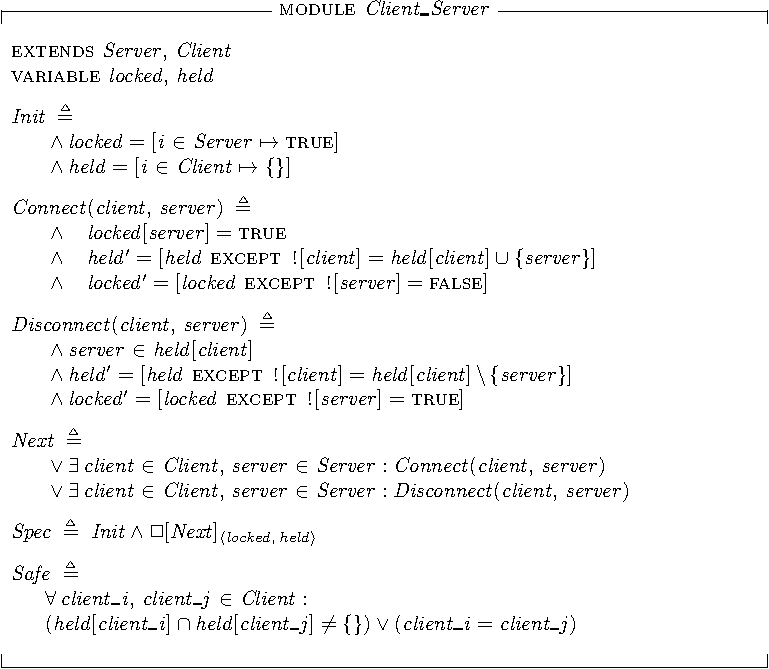
\includegraphics[width=0.8\textwidth]{figures/Client_Server.pdf}
    \caption{Client\_Server 规约}
    \label{fig:client_server}
\end{figure}

\section{\texorpdfstring{TLA\textsuperscript{+}与TLC}{TLA+与TLC}}
\subsection{\texorpdfstring{TLA\textsuperscript{+}形式规约语言}{TLA+形式规约语言}}
\href{https://lamport.azurewebsites.net/tla/tla.html}{\TLA} \cite{TLA+}是由计算机科学家 Leslie Lamport 主导开发的,基于时许逻辑TLA(temporal logic of actions)\cite{temporal}的,
在对计算机程序和系统建模,尤其是对并行系统和分布式系统建模具有广泛应用\cite{PaxosStore}的一种高级语言。
它是基于使用简单的数学语言来精确描述系统行为的理念开发的。
因此,\TLA 的表达方式和一般的编程语言有很大的不同,反而和数学语言更为接近。
\TLA 并不是一种编程语言,而是一种规约语言,它不关注协议或者系统的具体实现,从而能更高层次看到程序整体的设计。
因此,\TLA 及其工具对于消除代码中很难发现和纠错成本高昂的错误非常有用。

需要注意到的是,\TLA 是一个对程序或者系统建模的语言,为了让规约开发人员能更好地表达一个协议或系统而设计的,
并不是为了寻找归纳不变式而设计的。
尽管如此,它的语法更加丰富,以更加直观的方式表达一个协议或系统,而且在工业界应用更加广泛,使得它在寻找归纳不变式的研究中有广阔的应用。

开发者使用 \TLA 或者其他工具来对分布式协议进行建模的代码,我们将其称之为规约(specification,简称spec)。
图 \ref{fig:client_server} 展示了一个简单的 \TLA 规约,其中包含了一个简单的客户端和服务器的通信协议。
其中两个重要的谓词是 $Init$ 和 $Next$。
$Init$ 表示系统的初始状态,描述系统最开始时的状态;
而$Next$ 则是表示系统的状态是如何转移,也就是系统的状态在每个时间片后会发生怎样的变化。
谓词$Safe$ 是安全属性(safety property),一个正确定义的分布式协议规约,应当在每个可达的状态下都满足安全属性。
这个变量在自动化生成归纳不变式的研究中非常关键。
在这个规约中,还有$Connect, Disconnect$ 等这样的动作定义,使用这些定义,就像在一般的编程语言中使用函数一样,方便阅读和重复使用。
除此以外,一些规约中还有谓词 $TypeOK$,用于约束变量的类型。
另一种在自动归纳不变式生成研究中常常使用的工具,IVy,也有相似的语法和结构。
可以看到的是,\TLA 更关注系统的状态和系统状态是发生怎样的转移,对于系统状态转移的具体实现,\TLA 并不关心。
这样的描述方式和状态机非常相似。

TLC 是 \TLA 集成的模型检测工具。
除了 TLC 以外,\TLA toolbox\cite{tla+toolbox} 还集成有PlusCal\cite{PlusCal}和TLAPS用于命题证明工具,sany用于语法检查工具,
tex 用于将\TLA 美化打印的工具等,这些工具与本文所讨论的问题相关性不高,不展开讨论。

本文所述工具只接受\TLA 的规约。

\subsection{TLC模型检查器}\label{sec:tlc-apalache}
TLC既是对\TLA 规约的模型检查工具,也是一个面向规约的模拟器。
它是一个显式状态模型检查器,依照用户给出的规约和设置,搜索所有满足约束的状态和状态转移,
并在这个过程中检查安全属性和其他用户定义的谓词逻辑时时是否成立。
如果遇到错误,TLC会将错误的状态和状态转移过程输出,以便用户进行分析。

TLC可以通过使用超过32个计算机线程以获得近乎线性的加速。
它可以通过在分布式部署的计算机网络上运行来进一步加速模型检查,并提供在云系统上的轻松部署。

Apalache\cite{apalache1, apalache2}是另一由社区开发的模型检测器, 和 TLC 不同的是,Apalache 并不是通过遍历所有可能的状态来检验安全属性是否成立,而是通过 SMT solver 来检验。
它是将\TLA 规约转换为 SMT 问题,然后使用 SMT solver (如Z3\cite{z3})求解来检验安全属性是否成立。
Apalaches 是一种符号检查器,它和 SMT solver 一样基于逻辑推理和公式求解实现的。
Apalache 对\TLA 源文件的语法中引入了一些限制,
尽管没有完全支持\TLA 的所有语法,但是这方便使用 SMT 求解器进行求解。

\TLA 是一个“弱类型”的编程语言,它对变量没有严格的类型注明。
但是,Apalache 需要了解\TLA 规约中变量的类型才能工作。
尽管 Apalache 有一套自己的类型推断系统,但是,它并不能完全解决所有的类型推断问题。
这使得用户,对于某些协议,需要以注释的形式来提供变量的类型,才能交给Apalache进行处理。

\section{归纳不变式与归纳反例}
验证分布式协议的正确性,就是验证协议定义的安全属性(safety property)是否在每个可达的状态下都成立。
在 \textit{Client\_Server} 规约中,我们可以看到 $Safe$ 是一个安全属性,
它表达的是,在任何状态下,如果两个客户端同时连接有同一个服务器,那么这两个客户端是同一个客户端。
换言之,两个不同的客户端不能连接到同一个服务器。

对于简单的系统,即变量和状态不多的系统,我们可以通过遍历每一个可能的状态来验证。
但是对于稍微复杂一些的系统,尤其是越来越多的分布式系统,规模越来越大,状态也越来越复杂。
通过简单的遍历的方式来验证系统的正确性,是不现实的。
寻找一个能够蕴含安全属性的不变式,并且能够在所有可能的状态转移后保持其自身的正确性,这个不变式被称为归纳不变式。
以数学的语言表示为:
\begin{align}
    &Init \vDash Ind \label{con:init}\\
    &Ind \land Next \vDash Ind' \label{con:inductive}\\
    &Ind \vDash Safe \label{con:safety}
\end{align}
其中$Init$ 表示初始状态,$Next$ 表示状态转移,$Safe$ 是安全属性,$Ind$ 表达的是归纳不变式,
而$Ind'$表达谓词$Ind$经过状态转移后的变量的状态。
定理\ref{con:init}表明归纳不变式在初始状态下成立;
定理\ref{con:inductive}表明归纳不变式在状态转移后依然成立,具有归纳性质。
比如说,如果$Ind$在状态$s$下成立,那么在$s$的后继状态下,$Ind$依然成立;
定理\ref{con:safety}表明归纳不变式蕴含安全属性,因此,如果某个运行时可达状态满足$Ind$, 那么也必然满足$Safe$。
这是我们寻找一个这样的归纳不变式的目的,通过归纳不变式的正确性验证安全属性的正确性。
这是归纳不变式所必须满足的三个条件。

对于\textit{Client\_Server} 规约,表达式\ref{con:candidate_ind}是一个可能的归纳不变式。
\begin{align}
    &\left.A_{1} \triangleq \forall s \in  { Server }: \forall c \in  { Client }:  { locked }[s] \Rightarrow(s \notin { held }[c])\right) \\
    &{ Ind } \triangleq  { Safe } \wedge A_{1} \label{con:candidate_ind}
\end{align}

总结归纳不变式的特征,$Ind$是由$Safe$和$A_{1}$两个谓词逻辑表达式合取组成而来。
事实上,大部分规约的归纳不变式都可以表达为$Ind \triangleq Safe \wedge A_1 \wedge A_2 \wedge... \wedge A_n$的形式。
其中合取子式$A_k$是约束状态的谓词,我们将之称为引理不变式(Lemma Invariant)。
因为归纳不变式$Ind$是由这些引理不变式$A_k$组合而成的,也就是说,归纳不变式强于每一个引理不变式。
因此,引理不变式需要满足不变性,也就是在系统运行的每个状态下都成立,才能成为一个合适的引理不变式。
但是,引理不变式本身不需要满足归纳性,只需要它们和安全属性的合取结果能够满足归纳性。

对于一个谓词表达式$P$,如果一个状态$s$满足$s \models P$,但是$s$的后继状态$s_{n} \models \neg P$,
那便可以称$s$ 为 $P$的归纳反例(counterexample),揭示了$P$不是归纳不变式。
一个归纳反例往往包括两个状态,前一个状态满足谓词$P$,而后一个状态不满足谓词$P$。

\begin{figure}
    \centering
    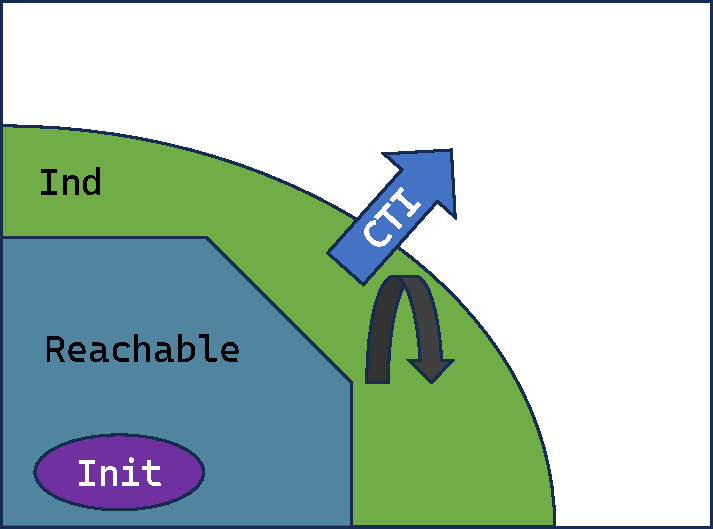
\includegraphics[width=0.4\textwidth]{figures/ind_cti.pdf}
    \caption{归纳不变式和归纳反例}
    \label{fig:ind-cti}
\end{figure}
图\ref{fig:ind-cti}形象地介绍了归纳反例以及归纳不变式、运行时可达空间和初始化空间之间的关系。
寻找归纳不变式的过程,也可以理解为通过添加新的引理不变式作为约束修剪空间,来排除归纳反例的过程。
但是,尤其是对于越复杂的系统而言,寻找归纳不变式并不是一个简单的任务。
实现归纳不变式的自动生成是形式化验证领域一个重要的研究目标,这也是本文研究的内容。

% 补充关于 返回结果和CTI的内容?

\section{强化学习}
强化学习(Reinforcement learning, RL)\cite{rl}是机器学习的一个领域,强调如何基于外部环境做出决策,以获得最大化的预期累积奖励。
是区别于监督学习和非监督学习的另外一种基本的机器学习方法。
强化学习的关注点在于寻找对未知领域的探索和对已有知识的利用之间的平衡。
它的目标是通过奖惩来控制智能体完成任务,以获得最大化的预期累积奖励,但程序无需明确告诉智能体如何完成任务。

在机器学习问题中,环境通常被抽象为马尔可夫决策过程(Markov decision processes,MDP)\cite{markov},
因为很多强化学习算法在这种假设下才能使用动态规划的方法。
但是,强化学习相较于动态规划,并不一定需要了解MDP的具体信息和全局信息,只需要通过与环境的交互,不断试错来学习。

\begin{figure}[h]
    \centering
    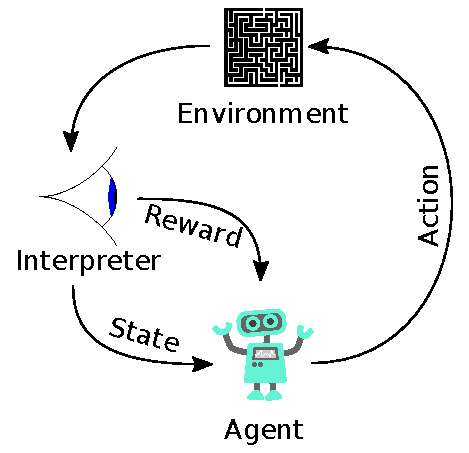
\includegraphics[width=0.4\textwidth]{figures/Reinforcement_learning_diagram.pdf}
    \caption{典型强化学习框架}
    \label{fig:rl}
\end{figure}
图 \ref{fig:rl} 展示了强化学习的框架。
在强化学习中,核心在于智能体(agent)与环境(environment)之间的交互。
环境是智能体所在的背景,它会根据智能体的动作给予奖励或惩罚,并做出状态的转移。
智能体能够感知环境的状态(State),并根据反馈的奖励(Reward)或惩罚(Reward为负值),来调整自身策略(Policy),
学习选择适当的动作(Action),以最大化长期总收益。
通过不断与环境互动,智能体根据环境的反馈不断调整策略,以期获得最大化的预期累积奖励。
实现强化学习的策略算法有很多,其中最著名的有 Deep Q Network(DQN)\cite{dqn},DDPG\cite{ddpg}等。

在本文的项目中,我们使用强化学习的方法来加速归纳不变式的生成。
我们使智能体理解\TLA 原文件的内容,让智能体合理选择生成归纳不变式的种子(seed),
并将每一次智能体选择的种子所生成的不变式的检验结果反馈给智能体,包括反例的数量,内容和生成时间等。
智能体根据这些反馈信息,调整自己的策略,以便更快地找到一个满足安全属性的归纳不变式。



\chapter{总结与分析}\label{chap:conclusion}
本章对论文工作进行了总结,并展望了未来可能的优化和改进方向。
\section{工作总结}
本文主要目的是验证机器学习,尤其是强化学习在对分布式系统规约的归纳不变式生成领域中的可行性和有效性。

本文在\TLA 的语言平台上,实现了一个基于强化学习的归纳不变式生成系统。
首先,介绍了系统设计的预备知识和理论基础,然后介绍了\rltla 的系统体系结构的设计和实现,最后展示了运行数据,并对结果进行分析。

\TLA 相较于 IVy 更加复杂,其中存在灵活多样的数据结构,同时也支持任意的嵌套来表达规约。
这对开发人员在设计阶段表达系统的行为和状态转移关系提供了很大的便利,但这点对于归纳不变式生成工具的设计并不友好。

实现上,本文依靠于\TLA 源文件和 endive 对于\TLA 解析和人工识别的假设作为输入,基于 try-and-error 的生成思路,
采用强化学习的方式生成候选不变式,通过模型检查器验证候选不变式的正确性,独立性以及当前所有候选不变式合取结果的递归性,最终生成归纳不变式。
这一生成思路和大部分的归纳不变式生成工具类似,但是在实现上,本文寄希望于强化学习以提高生成效率。

本文基于LIPuS \cite{LIPuS} 对结构化程序寻找循环不变式的研究开发了一套面向\TLA 的强化学习模型。

本文使用TLC和Apalache对生成的候选不变式进行验证,检验生成的候选不变式的正确性,独立性和与已有不变式合取结果的递归性,并将结果返回给强化学习模块。
TLC和Apalache没有提供python的接口,本文通过调用命令行的方式调用TLC和Apalache,并通过对命令行结果的解析,获取验证结果。

在测试部分,本文使用 endive 提供的测试用例对系统进行测试,并和endive进行了比较,
验证了强化学习在面向分布式系统规约的归纳不变式生成工作中具有可行性和有效性。

\section{未来展望}
由于时间和能力的限制,本文所实现的系统的性能和实现方式上有许多不足,存在大量的改进空间。

目前,和endive一样,\rltla 还以来于一些人工的输入,即一些人工识别的假设(predicates)
,这些假设的得到是依赖于人脑对于 \TLA 规约理解,尤其是对每个 Action 进行调用时参数类型的理解。
如果要自动化地识别和生成这些假设,也是一个复杂的工作,目前系统还不具备这项能力。
与此同时,人脑的参与可能带来效率的下降和不可预计的错处的出现。
另一方面,如同 endive 的通过机械搜索的方式,可能获得比强化学习更快的生成效率,强化学习的优势难以发挥。
未来需要实现一个功能更加丰富的静态分析工具,以自动提取出 \TLA 规约的语义信息,包括 Action 的"函数签名"等,
以帮助强化学习模块更好地理解 \TLA 规约和生成合适的候选不变式。

近些年,大语言模型的流行,使得自动归纳不变式生成有了更多可能。通过将协议交给大语言模型进行学习,可以更好地理解协议的行为。
或者,大语言模型也许可以直接应用于归纳不变式的生成工作,这是一个值得尝试的方向。

其次,目前提供给系统可以选择的谓词对于系统来说都是平行的,并没有考虑谓词的子式以及谓词之间的关系。
系统也无法考虑给出的这些谓词表达式之间,以及每个可能的候选不变式之间的关系。
这有可能导致系统生成的候选不变式之间存在冗余,或者存在矛盾,导致系统的效率降低。
另外,目前系统设计上,一次只生成一个可能的候选不变式,
这两方面因素,导致了对于每一次的生成的候选不变式的检查,都需要调用1-3次模型检查器进行检查,这往往很花时间,导致系统的效率较低。
这也是目前在效率上较 endive 等工作有所不足的地方。

基于\TLA 的归纳不变式的生成是一个复杂的问题,在这一领域的研究不是十分充足,可以参考和对比的工作较少。
目前,对于基于\TLA 的归纳不变式生成工具还没有统一的测试集合,也没有十分充足的测试用例。
这导致我们一方面很难评估系统的效率,另一方面,也很难提供给强化学习模块足够的训练数据。
在 endive 的测试集合下,一个归纳不变式常常只需要不超过10个子式合取而来。
在这一背景下,强化学习的效率并不理想,常常带来相较于 endive 等工作提供的搜索算法更高的开支和更低的效率。



% 生成参考文献页
\printbibliography

\begin{acknowledgement}
    致谢
\end{acknowledgement}

\end{document}